\newpage
\section{Suggested solutions: Arbitrary Frequency Response Filters}
\begin{enumerate}
\item Consider two signals of the form:
\begin{align*}
    x_{1}[n]&=\sum_{i=1}^{5}A_{i}\cos(2\pi f_{i}i)+w_{n}, \\
    x_{2}[n]&=a_1\delta[n-8192] + a_2\delta[n-9192] + a_3\delta[n-7192],
\end{align*}
where $|A_{i}|>|a_{j}|$ for every pair $i,j$, here $w_t$ is white noise.\footnote{White noise is considered as a random variable with a normal distribution corresponding $\mu=0$ and variance $\sigma^{2}=1$ here} In Listing \ref{code16_1} is code to generate these signals and plot them. 
\begin{lstlisting}[language=Python, caption=Example signal code,label=code16_1]
import numpy as n
import matplotlib.pyplot as plt

N = 16384
nn = n.arange(N)
freqs = [0.0003,0.012,0.055,0.102,0.85] # x1[n] frequencies
A = [1e5,5e5,1e3,1e4,0.5e4]             # x1[n] amplitudes
x1 = n.zeros(N)

# create the first signal
for i,f in enumerate(freqs):
    x1 += A[i]*n.cos(n.pi*freqs[i]*nn + n.random.randn(1))

# create the second signal (the weak signal)
x2 = n.zeros(N)
x2[int(N/2)] = 10.0
x2[int(N/2)+1000] = -5.0
x2[int(N/2)-1000] = 1.0

x = x1 + x2

# plot the signals
plt.plot(nn,x)
plt.xlabel("Samples")
plt.ylabel("$x[n]$")
plt.show()
\end{lstlisting}

\begin{marginfigure}
    \centering
    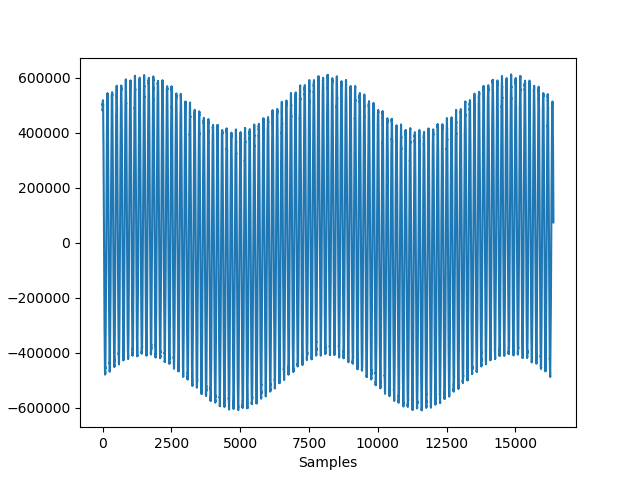
\includegraphics[width=7.5cm,height=7.2cm]{ch17/figures/ex16_1.png}
    \caption{Noisy signal we want to filter}
    \label{fig16_1}
\end{marginfigure}

\begin{enumerate}[a)]
\item To estimate the spectrum, we use the Hann window to avoid spectral leakage. 
The code for computing the spectrum using the Hann window is shown in Listing \ref{code16_2}.

\begin{lstlisting}[language=Python, caption=Spectrum for noisy signal in Figure \ref{fig16_1},label=code16_2]
import numpy as n
import matplotlib.pyplot as plt
import scipy.signal as ss

# function to convert to dB
def convert_to_decibel(x):
    return 10*n.log10(n.abs(x)**2)
    
N = 16384
nn = n.arange(N)
freqs = [0.0003,0.012,0.055,0.102,0.85] # x1[n] frequencies
A = [1e5,5e5,1e3,1e4,0.5e4]             # x1[n] amplitudes
x1 = n.zeros(N)

# create the first signal
for i,f in enumerate(freqs):
    x1 += A[i]*n.cos(n.pi*freqs[i]*nn + n.random.randn(1))

# create the second signal (the weak signal)
x2 = n.zeros(N)
x2[int(N/2)] = 10.0
x2[int(N/2)+1000] = -5.0
x2[int(N/2)-1000] = 1.0

x = x1 + x2

w = ss.hann(N)  # Hann window to reduce spectral leakage

xw = n.fft.rfft(w*x,2*N)    # use FFT to compute the spectrum
om_freqs = n.linspace(0,n.pi,num=len(xw)) # partition the interval (0,pi)

plt.plot(om_freqs,convert_to_decibel(xw))
plt.xlabel("$\hat{\omega}$ (rad / sample)")
plt.ylabel("$|\hat{x}_{w}[k]|^{2}$ (dB)")
plt.title("Spectrum of $x[n]$")
plt.show()
\end{lstlisting}

\begin{marginfigure}
    \centering
    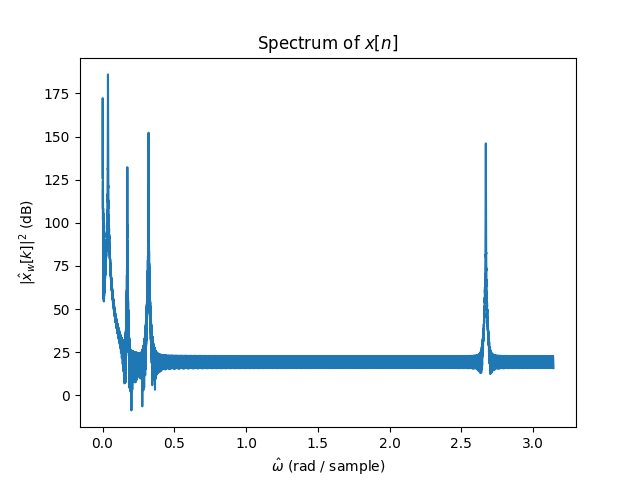
\includegraphics[width=7.5cm,height=8.0cm]{ch17/figures/ex16_2.png}
    \caption{Spectrum in dB for the signal shown in Figure \ref{fig16_1}}
    \label{fig16_2}
\end{marginfigure}

\item To filter out the noise, we use a filter that will remove strong spectral components and keep the 
weak components constant at $1.0$. That is, our filter will be:
$$\hat{h}[k]=\begin{cases}
    \frac{1}{|\hat{x}_{w}[k]|}, \quad \text{for strong spectral components}, \\
    1, \quad\quad \text{otherwise}.
\end{cases}$$
Where $\hat{x}_{w}[k]$ is the Hann windowed tapered signal. Looking at the spectral power, we can determine which components need to be lowered. 
After doing this we apply the inverse DFT to obtain our filtered signal,
$$x[k]=\mathcal{F}_{D}^{-1}\{\hat{x}_{w}[k]\hat{h}[k]\}.$$
The implementation of this is shown in Listing \ref{code16_3}.

\begin{lstlisting}[language=Python, caption=Filtering of the signal,label=code16_3]
import numpy as n
import matplotlib.pyplot as plt
import scipy.signal as ss

# function to convert to dB
def convert_to_decibel(x):
    return 10*n.log10(n.abs(x)**2)

N = 16384
nn = n.arange(N)
freqs = [0.0003,0.012,0.055,0.102,0.85] # x1[n] frequencies
A = [1e5,5e5,1e3,1e4,0.5e4]             # x1[n] amplitudes
x1 = n.zeros(N)

# create the first signal
for i,f in enumerate(freqs):
    x1 += A[i]*n.cos(n.pi*freqs[i]*nn + n.random.randn(1))

# create the second signal (the weak signal)
x2 = n.zeros(N)
x2[int(N/2)] = 10.0
x2[int(N/2)+1000] = -5.0
x2[int(N/2)-1000] = 1.0

x = x1 + x2

w = ss.hann(N)  # Hann window to reduce spectral leakage

xw = n.fft.rfft(w*x,2*N)    # use FFT to compute the spectrum
om_freqs = n.linspace(0,n.pi,num=len(xw)) # partition the interval (0,pi)

# define a filter to reduce strong spectral components
h = n.ones(len(xw)) # initialize each entry to 1

# lower the strong spectral components
# look at the previous exercise output plot to determine the intervals
# alternatively, plot the spectrum with samples on x-axis instead of \hat{\omega}
h[0:1050] = 1.0/n.abs(xw[0:1050])
h[1500:1860] = 1.0/n.abs(xw[1500:1860])
h[13500:14200] = 1.0/n.abs(xw[13500:14200])

# plot the spectral power to compare the two signals
plt.plot(om_freqs,convert_to_decibel(xw),label="Original spectrum")
plt.plot(om_freqs,convert_to_decibel(xw*h),label="Windowed spectrum")
plt.xlabel("$\hat{\omega}$ (rad / sample)")
plt.ylabel("Power of spectrum (dB)")
plt.legend()
plt.show()

# finally, inverse DFT to obtain the filtered signal
filter_signal = n.fft.irfft(h*xw)
plt.plot(filter_signal)
plt.xlabel("Samples")
plt.title("Filtered signal")
plt.show()
\end{lstlisting}
Running this code will generate the plots shown in Figure \ref{spectral_pw16} and \ref{filtered_signal}.

\begin{marginfigure}
    \centering
    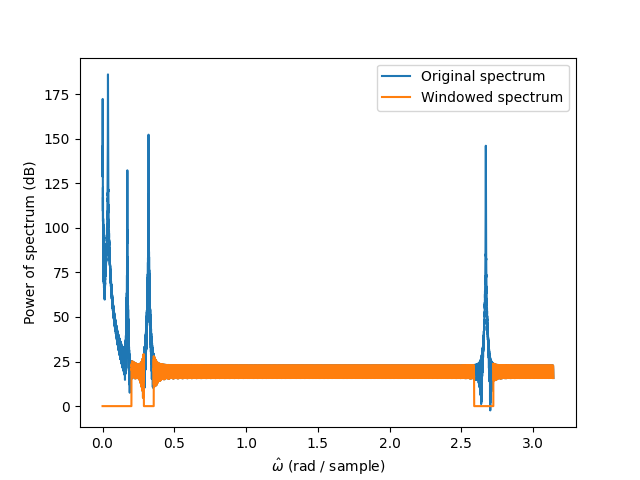
\includegraphics[width=7.5cm,height=7.0cm]{ch17/figures/spectral_pw.png}
    \caption{The comparison of the spectral power}
    \label{spectral_pw16}
\end{marginfigure}

\begin{figure}
    \centering
    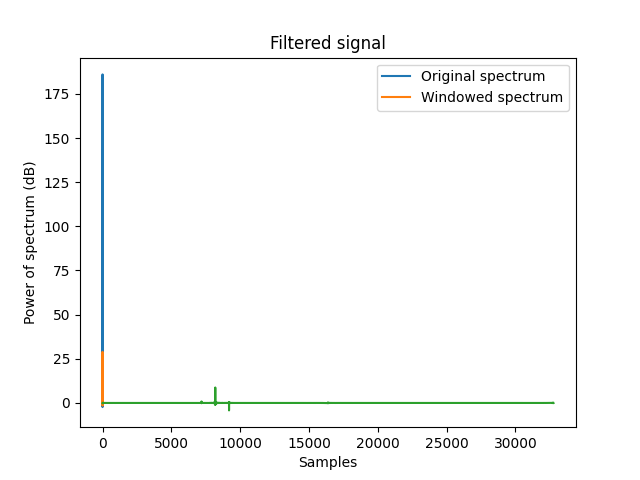
\includegraphics[height=9.0cm]{ch17/figures/filtered_signal.png}
    \caption{Filtered signal, the weak signal is now visible}
    \label{filtered_signal}
\end{figure}

\item The filter in this case reduces the strong frequencies while at the same time keeping lower frequencies fixed. The effect is that the original signal which had a lot of noise coming from $x_{1}[n]$ will have that noise significantly reduced. The remaining information in the signal is the other part, being $x_{2}[n]$, which consists of unit impulses for which the frequency components were kept at $1$. 
Therefore, the filtered signal looks like $x_{2}[n]$ even though a lot of frequency components have been removed. 
\end{enumerate}


\end{enumerate}